% Please do not delete!  thanks! -- zach
% !TEX root = ../../main.tex

\section{Evaluation Plan}
In this section, we will talk about methods to evaluate our solutions. This including two parts: methods used to evaluate our topic learning model and methods used to evaluating textbook suggestions which is our final product. 

\subsection{Evaluating Topic Modeling}
In order to carry out a comparative evaluation for a set of candidate recommendation algorithms, evaluation metrics will be used to measure some quality and performance features, in our case, we will use prediction accuracy to evaluate the models. The most popular metric that is used for evaluating prediction accuracy is Root Mean Squared Error (RMSE). RMSE is used measure of the differences between values (sample and population values) predicted by a model or an estimator and the values actually observed.  We will need to run this RMSE analysis on a data set with labels, and we are currently evaluating available data sets on Kaggle for fitness for this task.  
\newline
\begin{equation}
   RMSE = \sqrt{\frac{\sum_{1}^{n}\left ( \widehat{y_i}-y_i \right )^{2}}{n}}
\end{equation}
   
%i.	Surveying?
%ii.	Build a UI to present a book and a topic that was thought to be in the book
%iii.	User validates yes/no
%iv.	We use that feedback to tweak parameters of our models and to identify how many iterations of training we need to do (both our algorithms improve with more iterations)
\subsection{Evaluating textbook suggestions}
\subsubsection{Pre-Surveying}
To evaluate our project idea, we conducted a pre-surveying to see what the problem we are facing and how people reacting about our proposed solution. We asked our participants how long they will spend on find the right textbook, what aspect do they think is most important when choosing a textbook (except the content, our learning model will do the best of this part). See Table \ref{Pre-survey} for a breakdown of the questions to ask.

\begin{table}[ht] 
\caption{Questions in Pre-survey}
\label{Pre-survey}
\begin{center}
\begin{tabular}{ll}
\multicolumn{1}{c}{\bf Questions} 
\\ \hline \\
1. Are you a student or professor?\\
2. How much time do you spend on choosing a textbook?\\
3. How do you choose a textbook?\\
4. What aspect do you think is most important\\
when choosing a textbook (except the content)? \\
5. Would you consider an app that will give you \\
recommended textbooks base on your course \\
syllabus and your preference? \\
\end{tabular}
\end{center}
\end{table}
Among the 29 responses, we found that 73.3\% responded as they interested to our application to recommend the textbooks. The answer to most important aspect during the textbook chosen, review/ratings and sell price were the highest concern. These preliminary results give us the guidance to design the application and to improve the core learning models.
%\usepackage{graphicx}
%\graphicspath{ {/sections/eval_plan/} }
%\begin{figure}[ht]
%\caption{result of preSurvey}
%\centering
%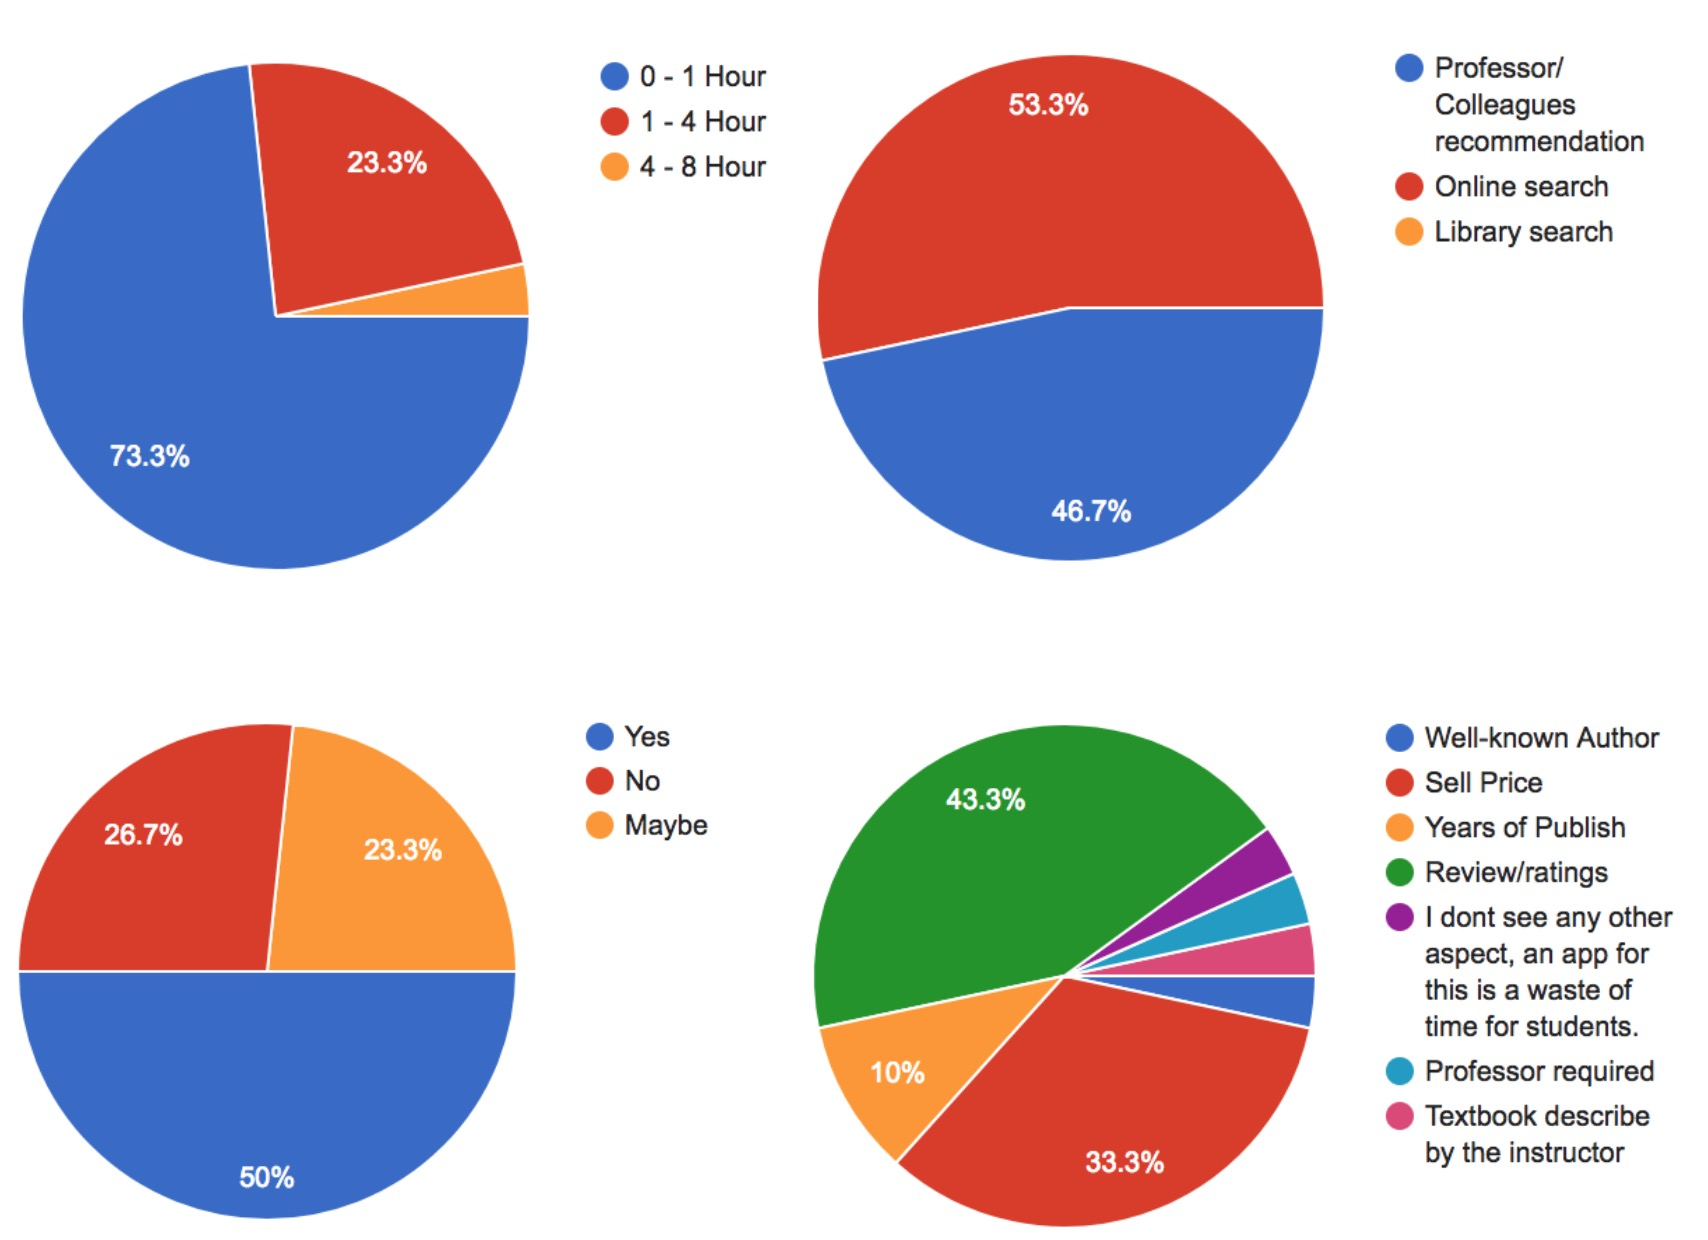
\includegraphics[width=0.5\textwidth]{preSurvey}
%\end{figure}
\subsubsection{Experiments}
\paragraph{Surveying Suggestions}
We have briefly discussed how we intend to validate that our model suggests books well and the usefulness of our application overall, but we have not yet discussed how we intend on validating whether or not the textbook recommendations that our algorithm make are topical (cover the topics) and are frugal (are less expensive than other options).  
To do this, we intend to do some focus grouping easier by some custom UI in our web app.

We intend to sit down a group of volunteers with our app and to give them access to our app with an anonymized user.  
They will be asked to find an appropriate textbook for a class using a provided list of topics.  
After choosing the appropriate topics and setting their own weighting on frugality and topic coverage, they will be asked to parse the results and rank their fitness for the particular purpose on a scale from $1$ to $5$ (with $5$ being perfect fit) and rate their cost from $1$ to $5$ (with $5$ being perfectly inexpensive compared to the alternatives).  
After rating the books that were suggested, the user will then be presented with the top 5 books that did not make the suggestion cut, and will be asked if any of these books should have replaced books that were presented and why they should have been on the list (for example, was the book expensive, but did it offer better topic coverage, or was there something unique about it that we should factor into our analysis).  
The test can then be repeated with the other algorithm.

This test will answer several questions.  
First, it allows us to evaluate if the topic mining is finding semantically appropriate items.  
By presenting the user with the top choices, then choices that were not considered optimal, we are attempting to see if the algorithm should have found a different book more relevant.  
We are also attempting to see if a book that was more or less expensive should have been on the list.  
More importantly, though, by rating suggestions on a 1 to 5 scale, we can easily compare the ratings of suggestions made by LDA to the ratings of suggestions made by Doc2Vec to see if there is a significant difference between them.  


%i.	Surveying?
%ii.	User selects topics they want to search for
%iii.	App presents 3 answers: 
%1.	an expensive but complete solution,
%2.	an inexpensive but incomplete solution,
%3.	a middle-of-the-road solution
%iv.	User identifies if the solutions are reasonable
%v.	User is presented with more (how many) books that did not make the cut, and is asked if one of those should have been in the top 3.  


